\documentclass[12pt]{scrartcl}


\setlength{\parindent}{0pt}
\setlength{\parskip}{.25cm}

\usepackage{graphicx}

\usepackage{xcolor}

\definecolor{darkred}{rgb}{0.5,0,0}
\definecolor{darkgreen}{rgb}{0,0.5,0}
\usepackage{hyperref}
\hypersetup{
  letterpaper,
  colorlinks,
  linkcolor=red,
  citecolor=darkgreen,
  menucolor=darkred,
  urlcolor=blue,
  pdfpagemode=none,
  pdftitle={CSCE 156 Lab Handout},
  pdfauthor={Christopher M. Bourke},
  pdfsubject={},
  pdfkeywords={}
}

\definecolor{MyDarkBlue}{rgb}{0,0.08,0.45}
\definecolor{MyDarkRed}{rgb}{0.45,0.08,0}
\definecolor{MyDarkGreen}{rgb}{0.08,0.45,0.08}

\definecolor{mintedBackground}{rgb}{0.95,0.95,0.95}
\definecolor{mintedInlineBackground}{rgb}{.90,.90,1}

%\usepackage{newfloat}
\usepackage[newfloat=true]{minted}
\setminted{mathescape,
               linenos,
               autogobble,
               frame=none,
               framesep=2mm,
               framerule=0.4pt,
               %label=foo,
               xleftmargin=2em,
               xrightmargin=0em,
               startinline=true,  %PHP only, allow it to omit the PHP Tags *** with this option, variables using dollar sign in comments are treated as latex math
               numbersep=10pt, %gap between line numbers and start of line
               style=default, %syntax highlighting style, default is "default"
               			    %gallery: http://help.farbox.com/pygments.html
			    	    %list available: pygmentize -L styles
               bgcolor=mintedBackground} %prevents breaking across pages
               
\setmintedinline{bgcolor={mintedBackground}}
\setminted[text]{bgcolor={mintedBackground},linenos=false,autogobble,xleftmargin=1em}
%\setminted[php]{bgcolor=mintedBackgroundPHP} %startinline=True}
\SetupFloatingEnvironment{listing}{name=Code Sample}
\SetupFloatingEnvironment{listing}{listname=List of Code Samples}


\usepackage{tikz}
\usetikzlibrary{calc,shapes.multipart,chains,arrows}

\title{CSCE 156 -- Computer Science II}
\subtitle{Lab 11.0 - Linked Lists}
\author{~}
\date{~}

\begin{document}

\maketitle

\section*{Prior to Lab}

\begin{enumerate}
  \item Review this laboratory handout prior to lab.
  \item Read the following wiki entry on linked lists: \\
	\url{http://en.wikipedia.org/wiki/Linked_list}
\end{enumerate}

\section*{Lab Objectives \& Topics}
Following the lab, you should be able to:
\begin{itemize}
  \item Use Linked Lists to store/retrieve/manipulate large 
  	collections of objects
  \item Implement Java interfaces
\end{itemize}


\section*{Peer Programming Pair-Up}

To encourage collaboration and a team environment, labs will be
structured in a \emph{pair programming} setup.  At the start of
each lab, you will be randomly paired up with another student 
(conflicts such as absences will be dealt with by the lab instructor).
One of you will be designated the \emph{driver} and the other
the \emph{navigator}.  

The navigator will be responsible for reading the instructions and
telling the driver what to do next.  The driver will be in charge of the
keyboard and workstation.  Both driver and navigator are responsible
for suggesting fixes and solutions together.  Neither the navigator
nor the driver is ``in charge.''  Beyond your immediate pairing, you
are encouraged to help and interact and with other pairs in the lab.

Each week you should alternate: if you were a driver last week, 
be a navigator next, etc.  Resolve any issues (you were both drivers
last week) within your pair.  Ask the lab instructor to resolve issues
only when you cannot come to a consensus.  

Because of the peer programming setup of labs, it is absolutely 
essential that you complete any pre-lab activities and familiarize
yourself with the handouts prior to coming to lab.  Failure to do
so will negatively impact your ability to collaborate and work with 
others which may mean that you will not be able to complete the
lab.  

\section*{Linked Lists}

List ADTs provide functionality for dealing with collections of 
objects in an object-oriented manner.  In contrast to ``static'' 
arrays that have a fixed size and require the client code to do
the necessary ``bookkeeping'' of the array, a List ADT provides 
an interface to dynamically add, remove, and retrieve elements 
while abstracting (hiding) the details of how it does it.  In 
an array-based list, the list would internally resize the array 
as necessary.  In a linked list, elements are added by creating 
nodes and manipulating references. 

A linked list is typically implemented using nodes which contain 
elements and a reference to a another node (the ``next'' node).  
In general, a linked list maintains a reference only to a head 
node.  A small example of a linked list containing integers. 
 
\begin{figure}[h]
\centering
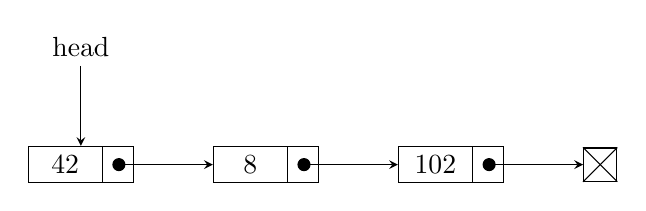
\begin{tikzpicture}[list/.style={text centered, text width=2em, rectangle split, rectangle split parts=2,
    draw, rectangle split horizontal}, >=stealth, start chain]

  \node[list,on chain] (A) {42};
  \node[list,on chain] (B) {8};
  \node[list,on chain] (C) {102};
  \node[on chain,draw,inner sep=6pt] (D) {};
  \draw (D.north east) -- (D.south west);
  \draw (D.north west) -- (D.south east);
  
  \node[above of=A,node distance=1.5cm] (H) {head};
  
  \draw[*->] let \p1 = (A.two), \p2 = (A.center) in (\x1,\y2) -- (B);
  \draw[*->] let \p1 = (B.two), \p2 = (B.center) in (\x1,\y2) -- (C);
  \draw[*->] let \p1 = (C.two), \p2 = (C.center) in (\x1,\y2) -- (D);
  
  \draw[->] (H) -- (A);
  
\end{tikzpicture}
\caption{A linked list with 3 nodes.  The head references the
first node while each node references the next node in the list, 
linking them all together.  The last node's next reference is
undefined (or null) or may point to a \emph{sentinel} node value
to indicate the end of the list.}
\label{figure:linkedList}
\end{figure}

In this lab, you will implement a linked list ADT that holds 
\mintinline{java}{Truck} objects and implements several standard 
methods.  Your list implementation is used in a larger inventory 
and truck management application, so you need to thoroughly 
test your implementation before you run the full application.

\section*{Activities}

Clone the starter code for this lab from GitHub using the following
url: \url{https://github.com/cbourke/CSCE156-Lab11}.

\subsection*{Linked List Implementation}

Most of the application code has been provided for you.  The 
\mintinline{java}{Truck} and \mintinline{java}{TruckListNode} 
classes representing trucks and a single node holding a truck has
been provided.  You will need to finish the implementation of the 
\mintinline{java}{TruckList} class.  

Specifically, you will first need to define the state of your list
and possibly a constructor.  Then you will need to implement the 
following methods.

\begin{itemize}
  \item \mintinline{java}{getSize()} -- This method returns the
  	number of elements in the list
  \item \mintinline{java}{clear()} -- This method will clear the 
  	entire list.  After calling it, the list should be empty
  \item \mintinline{java}{addToStart()} -- This method should add 
	the given truck to the front of the list
  \item \mintinline{java}{addToEnd()}  -- This method should add the 
	given truck to the end of the list
  \item \mintinline{java}{remove()} -- This method should remove the 
	truck at the specified position, assuming the list is indexed 
	starting at 0.  This method should throw an \\
	\mintinline{java}{IndexOutOfBoundsException} if an invalid 
	position is provided
  \item \mintinline{java}{getTruck()} -- This method should return 
	the truck at the specified position, assuming the list is indexed 
	starting at 0.  This method should throw an \\
	\mintinline{java}{IndexOutOfBoundsException} 
	if an invalid position is provided
  \item \mintinline{java}{print()} -- This method should print the 
	list to the standard output in a human readable format (hint: 
	make use of the \mintinline{java}{toString()} method).
\end{itemize}

You should look for opportunities where you can \emph{reuse} the
functionality of some of these methods rather than reimplementing 
the same algorithms.

\subsection*{Testing Your Implementation}

To make sure that your implementation works, you should utilize the 
utilities and other tools provided to design and write several test 
cases.  You will place these test cases into the 
\mintinline{java}{ListTester} class and make sure that the results are 
as expected.  You will need to write your own test cases.  As you 
write your test cases, keep the following in mind.

\begin{itemize}
  \item What are the ``corner case(s)'' that should be tested?  A 
	corner case is a pathological case that would occur only under 
	special circumstances and may require special consideration.
  \item Is it a good idea to test cases in which you know an exception 
	will be thrown?  Why or why not?  How could you test them?
  \item For this activity, a visual inspection suffices, but how 
	might you automate such testing to eliminate human error in the 
	process?  
\end{itemize}

To help you write test cases, a few tools have been provided to you.

\begin{itemize}
  \item The \mintinline{java}{ListTester} class gives you an example 
    of how to instantiate and use your \mintinline{java}{TruckList} class
  \item The \mintinline{java}{Truck} class has a static ``factory'' 
    method that creates a \mintinline{java}{Truck} with a random 
    license plate that you can use in your test cases
  \item The \mintinline{java}{Truck} class has a special idiom 
    (software design pattern) built into it: the \emph{builder pattern}.  
    The more member fields that an object has, the more difficult it is to 
    write consistent and readable code to call its various constructor(s).  
    The builder pattern allows you to use a \emph{fluent} style to 
    build an object by calling ``setters'' on an inner-builder class 
    prior to actually building the object.  Objects that have a builder 
    pattern are easier to use and construct.  The 
    \mintinline{java}{ListTester} class contains an example on how to 
    use the builder pattern.
\end{itemize}

\section*{Advanced Activity (Optional)}

The linked list you have implemented is constructed of nodes which 
can only contain instances of the \mintinline{java}{Truck} class. 
Modify the linked list to accommodate any type using generics. In 
simple terms, a generic can be thought of as a variable type. An 
example of a generic for an \mintinline{java}{ArrayList} is:

\mintinline{java}{ArrayList<MyType> listOfMyType = new ArrayList<MyType>();}

This statement constructs an \mintinline{java}{ArrayList} which 
only contains objects of \mintinline{java}{MyType}. You should 
rename your \mintinline{java}{TruckList} and \mintinline{java}{TruckListNode} 
to generic \mintinline{java}{MyList} and \mintinline{java}{MyListNode}.  
You then need to add a generic type to the implementation of 
\mintinline{java}{MyList} and \mintinline{java}{MyListNode} as follows.

\begin{minted}{java}
class MyList<T> { 
  ... 
}

class MyListNode<T> { 
  ... 
}
\end{minted}

The extra \mintinline{java}{<T>} at the end of these class definition 
indicates a generic type \mintinline{java}{T} will be used throughout 
each of these class definitions. When you need to construct a type of 
\mintinline{java}{T} in one such class you write:

\begin{minted}{java}
class MyListNode<T> {

  private T item;

}
\end{minted}

The \mintinline{java}{T} generic is a placeholder for the type which 
a use specifies. In the following code snippet a 
\mintinline{java}{MyListNode} is generated such that it can store 
objects of \mintinline{java}{MyType}:

\mintinline{java}{MyListNode<MyType> listNode = new listNode<MyType>();}

In your implementation of \mintinline{java}{print()} simply print 
out the string representation of the objects in your linked list 
using the \mintinline{java}{toString()} method of each object.

\end{document}
